%----------------------------------------
% Preamble to set up the document
%----------------------------------------
\documentclass{article}

% set up packages (you shouldn't need to touch this)
\usepackage{graphicx}  % required to insert images
\usepackage{hyperref}  % for hyperlinks
\usepackage[svgnames]{xcolor}  % to change hyperlink colors
\colorlet{linkcolour}{DarkBlue}
\hypersetup{colorlinks=true, linkcolor=linkcolour, citecolor=linkcolour, urlcolor=linkcolour,}
\usepackage{float}
% Margins
\topmargin=-0.45in
\evensidemargin=0in
\oddsidemargin=0in
\textwidth=6.5in
\textheight=9.0in
\headsep=0.25in

% use a sans serif font
\renewcommand{\familydefault}{\sfdefault}

%----------------------------------------
% Step 1: Edit the lecture title
%----------------------------------------
\title{
Lecture 8: Classification I - Naive Bayes \\  % Lecture title
Modeling Social Data, Spring 2017 \\   % Course title
Columbia University                    % School
}

%----------------------------------------
% Step 2: Edit your name and the date
%----------------------------------------
\author{Vedant Dharnidharka}                     % Scribe's name
\date{March 10, 2017}                % Lecture date

\begin{document}

\maketitle


%----------------------------------------
% Step 3:
% Rename uni.tex to match your uni,
% edit the filename accordingly below,
% and put your notes in this file
%----------------------------------------
%----------------------------------------
% Write your notes here
%----------------------------------------

\section{Classification}


Classification problem deals with categorization of given examples into a set of categories. 
\begin{figure}[H]
  \begin{center}
    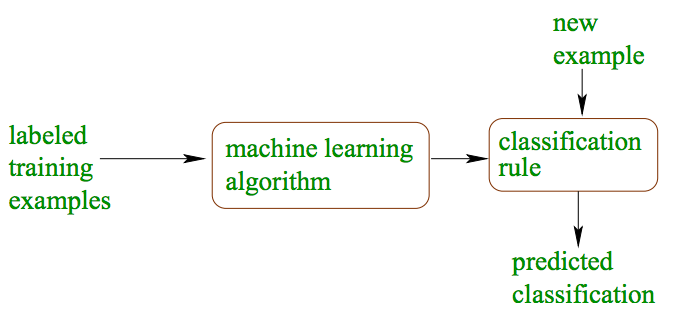
\includegraphics[width=0.5\textwidth]{classification.png}
    \caption{
      Classification}
  \end{center}
\end{figure}


\ 
\\{\itshape Input:} As with regression, in a classification problem we start with measurements {$x_1$, $x_2$, . . , $x_n$} in an input space $X$.
\\{\itshape Output:} \\
1. $Y$ = \{$-1$, +1\} or \{0, 1\} is called binary classification.\\
2. $Y$ = \{1, . . . , K\} is called multiclass classification.\\
Instead of a real-valued response, classification assigns x to a category. For pair ($x$, $y$), $y$ is the class of $x$.

\section{Naive Bayes Classifier}
The Naive Bayes classifier is based on the Bayes rule of conditional probability. It makes use of all the attributes contained in the data, and analyses them individually as though they are equally important and independent of each other. In some cases it is also seen that Naive Bayes outperforms many other comparatively complex algorithms.
\subsection{Bayes Theorem} A theorem describing how the conditional probability of each of a set of possible causes for a given observed outcome can be computed from knowledge of the probability of each cause and the conditional probability of the outcome of each cause.\\
\\Let ($\Omega$,P) be a probability space. ($\Omega$ is the sample space; P is the probability distribution.)
\\For any event A,B in $\Omega$
\\Formula: 
\begin{equation}
P(A|{B}) = P(A ) \frac{P({B} |A)}{P({B})},
\end{equation}
Let E, $H_0, H_1 $ in  $\Omega$. \\Conditioned on E, of $H_0$ and $H_1$, we find which one is more probable.
\\Compare $P(H_0) � P(E | H_0)$ to $P(H_1) � P(E | H_1)$
\subsubsection{Example}
\begin{figure}[H]
  \begin{center}
    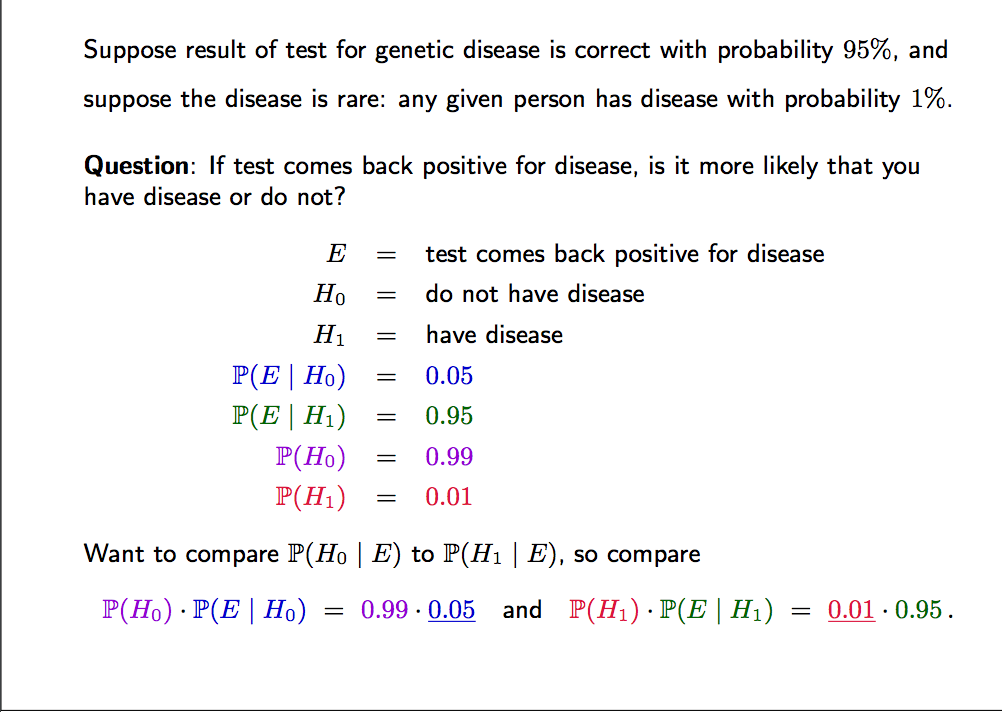
\includegraphics[width=0.5\textwidth]{disease.png}
    \caption{
      Bayes Theorem Example(Source: http://www.cs.columbia.edu/~djhsu/coms4771-f16/lectures/slides-generative.4up.pdf)}
  \end{center}
\end{figure}


\subsection{Maximum Likelihood Estimate}
\begin{figure}[H]
  \begin{center}
    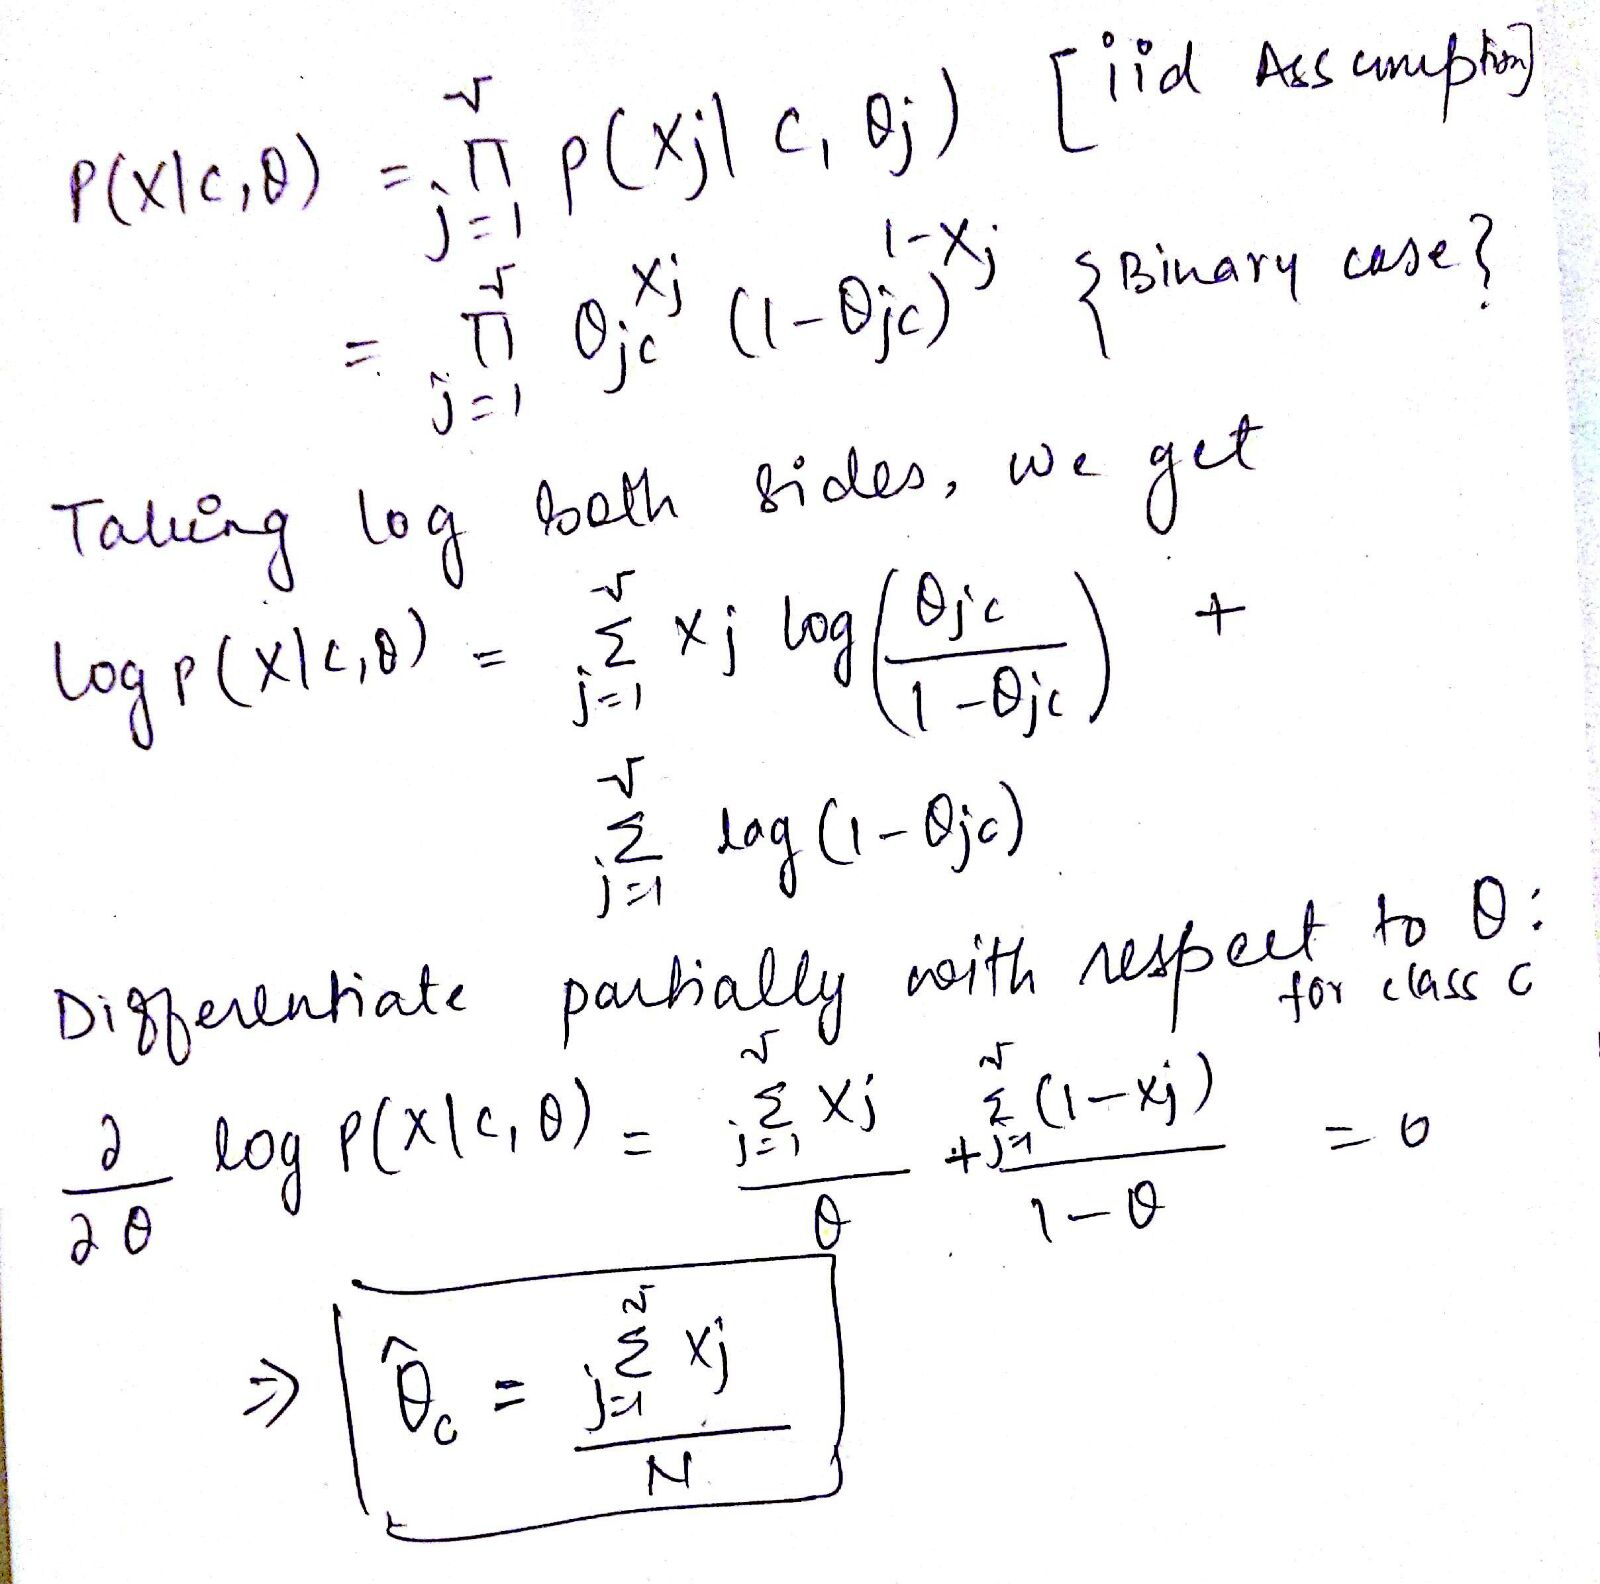
\includegraphics[width=0.5\textwidth]{mle.png}
    \caption{
      MLE for Naive Bayes}
  \end{center}
\end{figure}


\subsubsection{Advantages}
\begin{itemize}
    \item Simple, many variations
    \item Can leverage domain knowledge of class conditonals
    \item Can be very efficient when K is large.
\end{itemize}

\subsubsection{Disadvantages}
\begin{itemize}
    \item Classifier relies on formula (via Bayes\' rule) that assumes data comes from estimated distribution, which is generally not true.
    \item Modeling P away from decision boundary between classes is a wasted effort.
\end{itemize}

\section{Logistic Regression}
In logistic regression probability of the response taking a particular value is modeled based on combination of values taken by the predictors. 
\begin{figure}[H]
  \begin{center}
    \includegraphics[width=0.5\textwidth]{logr.png}
    \caption{
      Logistic Regression-Linear Classifier}
  \end{center}
\end{figure}

\subsection{Boosting}
Boosting is nothing but using a learning algorithm that provides rough rules-of-thumb to construct a very accurate predictor.\\
\\ Motivation: Easy to construct classification rules that are correct more-often-than-not (e.g., If over 5 percent of the e-mail characters are dollar signs, then its spam.), but seems hard to find a single rule that is almost always correct.\\
\\ Assumption: Availability of a base or weak learning algorithm which produces a weak classifier. Boosting improves the performance of the weak learning algorithm while treating it as a black box . Weak classifiers are not entirely trivial which means that  the error rates are at least a better than a classifier whose every prediction is a random guess. The weak classifiers can be moderately inaccurate, but not as bad as random guessing. \\
\\When they are added, they are typically weighted in some way that is usually related to the weak learners' accuracy. After a weak learner is added, the data are assigned weights again. Therefore when an entry is wrongly classified, the classifier which correctly classifies has its weight increased. 











\end{document}

%%% Local Variables:
%%% mode: latex
%%% TeX-master: t
%%% End: